\documentclass[12pt]{article}
\usepackage[brazil]{babel} % para relatórios em português
\usepackage[utf8]{inputenc} % para acentuação direta
\usepackage{amsmath,amsfonts,amssymb}  % improve math presentation
\usepackage{tabularx} % extra features for tabular environment
\usepackage{graphicx} % takes care of graphic including machinery
\usepackage[margin=0.8in,letterpaper]{geometry} % decreases margins
\usepackage[final]{hyperref} % adds hyper links inside the generated pdf file
\usepackage{xcolor}
%\usepackage[pdftex]{hyperref}

\hypersetup{
	colorlinks=true,       % false: boxed links; true: colored links
	linkcolor=blue,        % color of internal links
	citecolor=blue,        % color of links to bibliography
	filecolor=magenta,     % color of file links
	urlcolor=blue         
}

\begin{document}

\title{Manual Git/GitHub HigFlow}
\author{HigFlow e HigTree}
\date{\today}
\maketitle

\section{Configurações iniciais}\label{sec:configuracoes}
Para acessar o tutorial completo com as explicações mais detalhadas acesse \cite{site1}. As primeiras/recomendadas configurações para uso do \textit{Github}, deve-se (após instalado o \textit{git}) abrir um terminal e digitar:
\begin{itemize}
	\item \textbf{git config  -\hspace{0.5mm}-global user.name ``\textcolor{blue}{Your Name}"}
	\item \textbf{git config -\hspace{0.5mm}-global user.email \textcolor{blue}{your\_email\_github@example.com}}
\end{itemize}

Para acessar o tutorial completo acesse \cite{site2}. Para conseguir fazer alterações no GitHub do grupo deve-se registrar uma chave \textit{ssh} da máquina que você usa. 


Para criar uma nova chave \textit{ssh} da sua máquina, digite no terminal:
\begin{itemize}
	\item \textbf{ssh-keygen -t ed25519 -C ``\textcolor{blue}{your\_email\_github@example.com}"}
	\item \textbf{eval ``\$(ssh-agent -s)''}
	\item \textbf{ssh-add $\sim$/.ssh/id\_ed25519}
\end{itemize}
Ainda no terminal, para visualizar a chave pública recém criada, digite:
\begin{itemize}
	\item \textbf{cat $\sim$/.ssh/id\_ed25519.pub}
\end{itemize}
Este comando deve imprimir em tela algo parecido com:
\begin{itemize}
	\item[] ssh-ed25519 LetrasAleat0riasENumer0s7amb3m your\_email\_github@example.com
\end{itemize}
Copiei esta mensagem do seu terminal (essa é a parte publica da chave criada)! Posteriormente entre no seu GitHub no site e siga as seguintes instruções:

\begin{itemize}
	\item \textbf{Acesse: Settings \textrightarrow\quad SSH and GPG keys \textrightarrow\quad New SSH key }
	\item No campo \textbf{Title}, utilize um nome para identificar a máquina que está utilizando e no campo \textbf{Key} cole a mensagem gerada no terminal ao digitar o comando \textbf{cat $\sim$/.ssh/id\_ed25519.pub}. Abaixo seguem algumas imagens dos passos acima:
\end{itemize}
\newpage
\begin{figure}[htb]
	\centering
	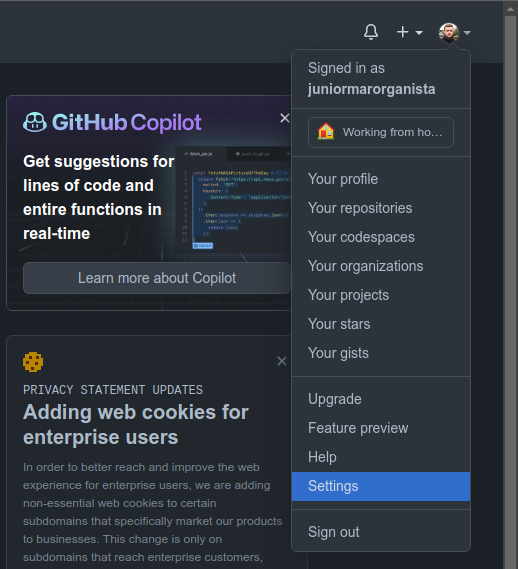
\includegraphics[width=0.4\linewidth]{figures/ssh_1}
	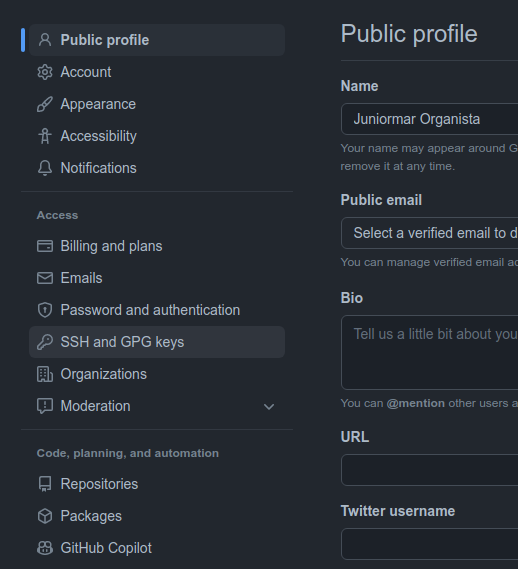
\includegraphics[width=0.4\linewidth]{figures/ssh_2}
\end{figure}

\begin{figure}[htb]
	\centering
	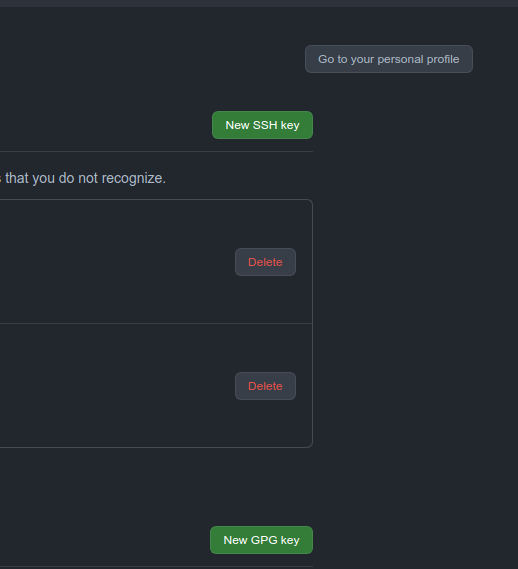
\includegraphics[width=0.4\linewidth]{figures/ssh_3}
	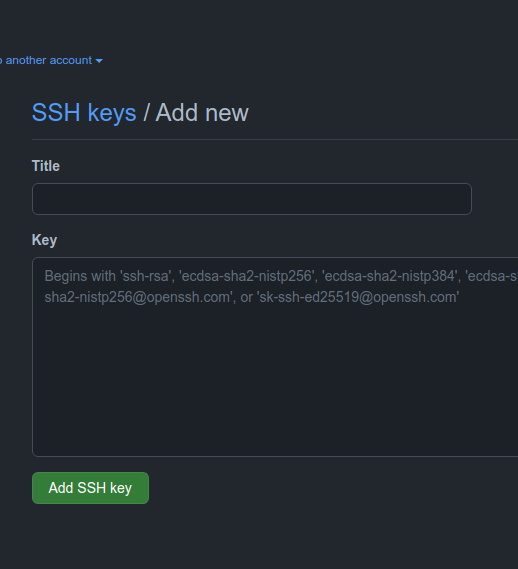
\includegraphics[width=0.4\linewidth]{figures/ssh_4}
\end{figure}

Essas configurações servem para a maquina que foi criado a chave em questão. Caso utilize o projeto em mais de uma máquina, será necessário repetir esse processo na outra máquina. Na sua conta do GitHub terá todas as máquina que sua conta está associada. 
Existe ainda a possibilidade da máquina não suportar a tecnologia associada a criação da chave \textit{ssh} com o algoritmo \textit{\textbf{Ed25519}}. Caso isso ocorra, será necessário criar uma chave do tipo \textit{rsa}, para será necessário trocar a criação da chave de
\begin{itemize}
	\item \textbf{ssh-keygen -t ed25519 -C ``\textcolor{blue}{your\_email\_github@example.com}"}
\end{itemize}
por
\begin{itemize}
	\item \textbf{ssh-keygen -t rsa 4096 -C ``\textcolor{blue}{your\_email\_github@example.com}"}
\end{itemize}

\section{Projeto HigFlow no GitHub - Primeiro passos}\label{sec:github_higflow}

O primeiro passo para se ter acesso ao projeto HigFlow no GitHub é solicitar a permissão ao administrador do projeto, Prof. Dr. Antonio Castelo Filho, através do email: \textbf{castelo@icmc.usp.br}. Após receber o convite para o projeto e aceita-lo, siga os passos abaixo pra ter uma versão na maquina que deseja trabalhar (que já tenha realizado as instruções da seção \ref{sec:configuracoes}). Primeiramente abra um terminal no diretório que deseja baixar o projeto e digite o comando abaixo:
\begin{itemize}	
	\item \textbf{git clone git@github.com:antoniocastelofilho/HigFlow.git}
\end{itemize}

Para iniciar suas alterações no projeto é necessário que se crie um \textit{\textbf{Branch}}(ramo/versão) com algum titulo que identifique o usuário. Posteriormente quando possuir uma versão amplamente testada e estável será realizado um merge no código principal.

\section{Comandos básicos do Git para controle de versão}\label{sec:comandos_pc}

Alguns comandos de uso cotidiano (para maiores informações consulte \cite{site3}):

\begin{itemize}
	\item \textbf{git init} $:=$ Cria o controle de versões git na pasta.
	
	\item \textbf{git status} $:=$ Exibe o status dos arquivos controlados e não controlados.
	
	\item \textbf{git add -A} $:=$ Adiciona todos os arquivos da pasta para controle.
	
	\item \textbf{git add poisson.m} $:=$ Adiciona o arquivo 'poisson.m' pasta para controlar.
	
	\item \textbf{git add -u} $:=$ Adiciona somente os arquivos já adicionados e que foram modificados.
	
	\item \textbf{git commit -m ``\textcolor{blue}{Comentario da versao}"} $:=$ Faz os arquivos adicionados serem controlados pelo git e adiciona o comentário 'Comentario da versao'.
	
	\item \textbf{git checkout -b \textcolor{blue}{add-var-in-main}} $:=$ Cria um \textit{\textbf{Branch}}(ramo) com o nome 'add-var-in-main', que na pratica pode ser usado para voltar um determinado arquivo antes de algumas alterações. 
	
	\item \textbf{git checkout master} $:=$ Muda para o Branch denominado 'master'.
	
	\item \textbf{git merge teste\_merge -m ``\textcolor{blue}{teste de domingo}"} $:=$ Quando no Branch 'master' este comando unifica a versão contida no branch 'teste\_merge' ao 'master' com o comentário `teste de domingo'.
	
	\item \textbf{git log -\hspace{0.5mm}-oneline -\hspace{0.5mm}-decorate -\hspace{0.5mm}-all -\hspace{0.5mm}-graph} $:=$ Mostra um diagrama do estado de controle dos arquivos.
	
	\item \textbf{git config -\hspace{0.5mm}-global alias.tree ``log -\hspace{0.5mm}-oneline -\hspace{0.5mm}-decorate -\hspace{0.5mm}-all -\hspace{0.5mm}-graph"} $:=$ Cria o comando 'tree' que executa o comando 'log -\hspace{0.5mm}-oneline -\hspace{0.5mm}-decorate -\hspace{0.5mm}-all -\hspace{0.5mm}-graph'.
	
	\item \textbf{git tree} $:=$ Executa o comando `tree' criado.
	
	\item \textbf{sudo apt install gitk} $:=$ Instala um visualizador gráfico.
	
	\item \textbf{gitk} $:=$ Executa o visualizador gráfico.
	
	\item \textbf{git remote add origin \textcolor{blue}{https://github.com/your\_user/project.git}} $:=$ Usado para adicionar um 'origin' para o repositório se não existe nenhum.
	
	\item \textbf{git pull origin master} $:=$ Caso o 'origin' já esteja adicionado na pasta, este comando é usado para buscar e baixar conteúdo de repositórios remotos e fazer a atualização imediata ao repositório local.
	
	\item \textbf{git push -u origin master} $:=$ É usado para enviar conteúdo do repositório local para um repositório remoto.
	
	\item \textbf{git clone \textcolor{blue}{https://github.com/your\_user/project.git}} $:=$ É utilizado para selecionar um repositório existente e criar um clone ou cópia do repositório alvo (no caso GitHub).
	
\end{itemize}

\bibliographystyle{plain}
\bibliography{git.bib}

\end{document}
